
%%%%%%%%
\begin{figure}
\centering
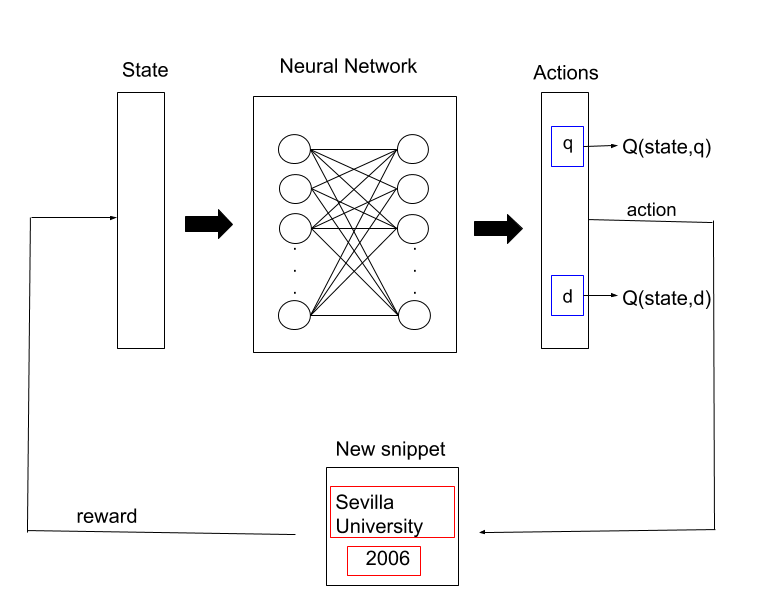
\includegraphics[scale=0.3]{./images/neural-network-3.png}
\caption{Deep Q-network framework for our web navigation system. If state input is a snippet (vector) the neural network is an LSTM ( regular densely-connected NN). }
\label{fig:model}
\end{figure}

%%%%%%%%%%

\begin{algorithm}[h]
 \small{
 \KwData{Initialize an experience replay memory $\mathcal{D}$ with $N$ capacity }
 \KwResult{$Q$-value function after training}
Initialize a Q-value function $Q$ with random weight $\theta$\\ 
 \For{episode $=0$ \KwTo $M$ }{
 	get a random person-id and initialise environment with start snippet $s_1$\\% state $s_1$
 \For{$t=1$ \KwTo $T$}{
	\eIf{random() $<\epsilon$}{ 
 	select a random action $a_t \in A$
 	}{$a_t = \text{argmax}_a Q(\phi(s_t), a; \theta)$}
Execute action $a_t$ and obtain reward $r_t$ and new snippet $s_{t+1}$\\
$\mathcal{D} \longleftarrow (\phi(s_t), a_t, r_t, \phi(s_{t+1})) \cup \mathcal{D}$\\
sample random mini-batch of transitions $(\phi(s_j), a_j, r_j, \phi(s_{j+1})) $ from $\mathcal{D}$\\
\eIf{$s_{j+1}$ is terminal}{
	$y_j = r_j$
}{
	$y_j = r_j + \gamma \text{max}_{a'} Q(\phi(s_{j+1}), a';\theta)$ 
}
perform gradient descent on the loss $L(\theta)$ based on $y_j$ \\
\If{$s_{t+1}$ is terminal}{
\textbf{break}}
}
}
\BlankLine
}
 \caption{Training Procedure via Deep Q-Network}
 \label{algo:qdn}
\end{algorithm}	
%%%%%%%%%%%%%

With the aim of extracting accurate name entities (containing organisation names and dates) and tracking experts we propose a Markov Decision Process (MDP) model and list of query types for searching the web using various search engines. Query types and the MDP model are explained in the following.

\paragraph{Queries: }  %Since \textit{unoporuno} is an intelligent web navigation system, it requires some search engines and query generation models.
For generating snippets and extracting information from them, we use five search engines including DuckDuckGo, Google, Bing, CiteSeerx and Researchgate .As the person name comes from an available database (supported by the sociologists), we generate $7$ possible number of queries for each name in each search engine: \\

$<$person name$>$ $+$ (  [] $|$ doctorate $|$ institute $|$ master $|$ undergraduate $|$ university ) 

\paragraph{Markov Decision Process: } Using a similar framework as Narasimhan et al. \shortcite{narasimhan2016improving}, we model our web navigator model as a Markov Decision Process (MDP) \cite{puterman1994}. The MDP parameters including States, actions and rewards are defined as below:

\begin{itemize}
	\item %The \textit{states} should be modeled in a way indicating the difference between the current and new snippets. 
	 We utilise two models of \textit{states} in this work regarding the Deep-Q network method and its contained neural network for computing the Q-value functions:
	\begin{itemize}
		\item \textit{Vector based}: each snippet is indicated with a vector of real values containing: \\
		-- one-hot $7$ encoding indicating which query type is used for generating the snippet,\\
	    -- one-hot $4$ dimensional encoding indicating which research engine is used, \\
		-- number of common organisation names and dates between gold standards for a given person and extracted name entities in the new snippet,\\
        -- confident score for extracted organisation names and dates. 
		\item \textit{text based}: Each snippet is considered as a state.
	\end{itemize}
	\item We have two \textit{Actions} including $q$ and $d$ indicating changing query and staying on the current query respectively. 
	\item The system goal is to extract the closest extracted organisation names and dates to the gold standards by generating less number of queries. For this reason, choosing the $q$ action in each state has a negative reward. And every time the extracted organisation name or date from a new snippet is close to the gold standards, the system receives a positive reward, for instance $r(s, q) = -0.1$ or $r(s, d) = 10$ if the extracted organisation name (year) is in the list of organisation names (years) for the gold standards. 
\end{itemize}

\paragraph{Algorithm}
A Deep Q-network (algorithm~\ref{algo:qdn}) demonstrates our approach for learning the experts professional tracks. 
In the initialization step, we start with a replay memory $\mathcal{D}$ storing transition examples $(s, a, r, s' )$ and a neural network for the $Q$-value function with random weights $\theta$. The whole training dataset is passed through for $M$ epochs. 

Referring to the model each new observed snippet should be presented as a state. The $\pi$ function in the algorithm signifies our utilised representation for a new observed snippets. According to Figure~\ref{fig:model} and the above explanation on the state representation, we have two models depending on the used neural network model for the Q-value function computation. 
\begin{itemize}
\item If $\phi$ is the vector representation, the neural network of our experiments is a regular densely-connected NN with $3$ layers. The first two layers use \textit{RELU} as their activation functions with a $0.25$ rate dropout for each, while the final layer has a \textit{linear} activation function. 
\item If $\phi$ keeps the snippet, the neural network of our experiments is a Long Short Term Memory (LSTM) (\question{that should be completed by Ivan})
\end{itemize}

From the feedback of environment in the form of rewards, the network parameters $\theta$ should be learned. To perform update of $\theta$, we keep an experience memory $\mathcal{D}$ for saving state transitions. In each backpropogation step, the $\theta$ parameters are calculated by sampling a mini-batch of transitions $(s', a', s'', r')$ at random from $\mathcal{D}$ and minimising the following loss function \footnote{The loss function is a mean square error function}:
$$L(\theta) = \mathbb{E}_{s', a'}[(y - Q(\phi(s'), a', \theta ))^2]$$
If we test the DQN algorithm, $y$ is calculated using two formulas in lines $14$ and $16$ from the algorithm~\ref{algo:qdn}. \PA{On the other hand we have some experiments with Dueling DQN (DDQN)\cite{wang2016} which is the same as the DQN except the line of $16$ in the algorithm. }

{\small{$$y_j = r_j + \gamma Q\left( \phi(s_{j+1}), \text{argmax}_{a'} Q(\phi(s_{j+1}), a';\theta); \theta^- \right)$$}}

\PA{To deal with the overoptimistic value estimation,the DDQN uses two neural networks for selecting the best action (with parameters $\theta$) and evaluating an action by computing Q-value function with $\theta^-$ pramaters from the previous iteration. }

\question{we will add a brief explanation for finishing on algorithms after being certain about the experiments.}



